% Replication Report Template
% Author: [Your Name]
% Date: [Date]

\documentclass{article}

\usepackage[a4paper, margin=1.0in]{geometry}
\usepackage{graphicx}
\usepackage{hyperref}
\usepackage[natbibapa]{apacite}
\usepackage{longtable}
\usepackage{booktabs}
\usepackage{amssymb}
\usepackage{amsmath}

\setlength{\parskip}{\baselineskip}


\title{Replication report of ``Productivity Shocks, Long-Term Contracts and Earning Dynamics'' by Balke \& Lamadon (2022)}
\author{Bruno Esposito}
\date{November 2023}

\begin{document}

\maketitle

\section{Introduction}

I replicate the results of the paper ``Productivity Shocks, Long-Term Contracts and Earning Dynamics'' by \cite{balke2022productivity}. The paper examines how employer- and worker-specific productivity shocks transmit to earnings and employment. The intricate dynamics between employer and worker productivity shocks and their transmission to earnings and employment remain a pivotal area in economic research. The work of Balke and Lamadon (2022) explores this complex relationship by developing an equilibrium search model that characterizes the optimal contracts offered by firms. Central to their analysis is the concept of risk-neutral firms providing partial insurance against productivity shocks to risk-averse workers, a mechanism that shapes earnings dynamics. The original study stands out for its empirical approach, utilizing matched employer-employee data from Sweden to estimate the model and its parameters.

The methodology of the original research involves a detailed characterization of the optimal contract in an equilibrium search model, accounting for both individual- and firm-level productivity shocks. This approach addresses risk-averse workers who lack commitment ability, a realistic aspect often observed in labor markets. The model, backed by Swedish data, enables the identification of productivity processes in a nonparametric manner. Key findings from the study include an analysis of various insurance channels and their interplay with worker incentives, quantification of the variance contributions from different uncertainty sources to wages, and the extent of productivity shock pass-through to workers. 



\begin{table}[ht]
\centering
\caption{Parameter Estimates}
\begin{tabular}{@{}lcc@{}}
\toprule
\textbf{Parameter} & \textbf{Estimate} & \textbf{Standard Error} \\
\midrule
Persistence for worker productivity & \(\lambda_x\) & 0.91 \\
& & (0.0053) \\
Persistence for match quality & \(\lambda_z\) & 0.95 \\
& & (0.0040) \\
Dispersion for worker permanent productivity & \(\sigma_{x_0}\) & 0.33 \\
& & (0.025) \\
Dispersion for worker transitory productivity & \(\sigma_{x_1}\) & 0.70 \\
& & (0.023) \\
Dispersion for match quality & \(\sigma_z\) & 0.49 \\
& & (0.015) \\
Effort cost parameter & \(\gamma_0\) & 0.00064 \\
& & (0.00031) \\
Effort cost curvature & \(\gamma_1\) & 0.37 \\
& & (0.015) \\
Flow payment while unemployed & \(b\) & 0.11 \\
& & (0.027) \\
Efficiency of the matching function & \(\alpha\) & 0.19 \\
& & (0.0024) \\
On-the-job search efficiency & \(\kappa\) & 0.53 \\
& & (0.024) \\
Measurement error on earnings & \(m_w\) & 0.20 \\
& & (0.0041) \\
Measurement error on value added per worker & \(m_y\) & 0.19 \\
& & (0.0039) \\
\bottomrule
\end{tabular}
\label{tab:parameters}
\end{table}


\section{Data}

The authors are able to track worker earnings, employment and unemployment spells, demographic and socioeconomic characteristics. They link each worker to the firm they are working on and measure the size and value added of each firm. The sample is composed by employer-employee matched data which links four Swedish administrative datasets: the Longitudinal Database of Education, Income and Employment (LOUISE), the Register-based Labor Market statistics (RAMS), the Structural Business Statistics (SBS) and the Unemployment Register. The authors consider the period 2001-2006. Self-employed individuals are removed from the sample. Additionally, the authors only consider males between 25 and 50 years old in order to remove labor participation decisions from the analysis. The sample includes around 1.2 million workers and over 70,000 firms.


\section{Replication}

The authors provide a public GitHub repository with the code required to replicate the paper. There are three main stages in their analysis. First, they compute a set of moments and data statistics from the administrative raw data. Second, they find the parameters that minimize the distance between the data moments and the moments simulated from the model. Third, they use the estimated parameters to simulate the model and run counterfactual analyses. The authors estimate that the second part of the analysis requires 600 core-hours and the third, 300 core-hours. 

\subsection{Stage 1: Data moments and statistics}

The first part of the analysis is straightforward. The authors calculate the selected moments using the Swedish employer-employee matched data. However, it cannot be replicated in this report because the dataset used is private. Regardless, the authors provide the values and standard deviations of the observed moments, as shown in table \ref{tab:moments_model_fit}. The remaining two parts of the analysis are replicated in this report.


\subsection{Stage 2: Model estimation}

The second part of the analysis focuses on estimating the parameters that minimize the distance between the observed moments in the data and the simulated moments from the model. The authors use simulated method of moments. There are four main steps in this procedure: model initialization, value function optimization, simulation of moments and parameter optimization.

\textbf{Initialization.} The authors specify values for 11 sets of primitives (Table \ref{tab:primitives}). Notice that some are hyperparameters which will not be optimized (e.g. the number of grid points for the productivity shocks). They estimate a simpler version of the model that features (i) no on-the-job search, (ii) fixed wages and (iii) optimization problem of the firm is not restricted by the worker's incentive constraint. In this simplified model, there are three bellman equations: the employed worker, the unemployed worker and the firm with a filled vacancy\footnote{The bellman equation of the vacant firm is not included due to the presence of the entry-free condition.}. Each one of these is approximated using value function iteration and used as initial value for the estimation of the full model.

\textbf{Value function optimization.} There are two main bellman equations to be approximated in the full model: the unemployed worker and the firm with a filled vacancy. The value function of the employed worker is not directly approximated anymore because the associated incentive constraint of the employed worker is included as a restriction in the maximization problem of the firm with a filled vacancy. Particularly, the optimal worker policies enter the firm's optimization problem via the retention probability $\tilde{p}(x, W)$ and the utility return $\tilde{r}(x, W)$. Recall that $x$ is the worker's productivity and $W$ is the promised lifetime expected utility to the worker. Notice that this feature adds another layer of complexity to the value function iteration problem, as firms need to incorporate the impact of $W$ on the worker's behavior. Finally, the bellman equations of the unemployed worker and the firm with a filled vacancy are approximated using value function iteration. 

\textbf{Simulation of moments.} After the model is solved, the authors draw a sequence of shocks for worker productivity and match quality. They simulate the choices of the agents using the optimal policy functions associated to the value function iteration. They repeat this process 20 times. Finally, they calculate the moments of interest from the simulated data.

\textbf{Parameter optimization.} The parameters of the model are optimized such that the weighted distance between the observed moments and the simulated moments in the smallest. At each iteration, the parameter is adjusted in the direction that reduces the distance between the simulated and observed moments. Then, the model is solved again, starting with the initialization step. The process is repeated 16 times. 
 

\section{Results}

The authors first show that the model is able to replicate the observed moments in the data (Table \ref{tab:moments_model_fit} shows the replicated table). Then, they run a set of counterfactual experiments. First, they evaluate the impulse responses to a permanent shock on the worker productivity $x$ (Figure \ref{fig:impulse_response_x}) and the match quality $z$ (Figure \ref{fig:impulse_response_z}). Both figures are successfully replicated. Second, the variance of math output, target wage and earnings is decomposed into three elements: permanent worker productivity, transitional worker productivity and match quality. Table \ref{tab:level_variance_decomposition} and Table \ref{tab:growth_variance_decomposition} show the replicated results. Third, the authors implement a pass-through analysis of a persistent worker productivity shock and match quality shock onto the utility and wage of the worker. Table \ref{tab:pass_through} shows the replicated results. Finally, the authors also show a counterfactual analysis of the impact of a change in the tax system. Unfortunately I was not able to replicate this final result with the code provided.

\begin{table}[ht]
\centering
\caption{Moments and Model Fit}
\begin{tabular}{@{}lcc@{}}
\toprule
& \textbf{Data} & \textbf{Model} \\
\midrule
\( Pr^{U2E} \) & 0.17 & 0.16 \\
& (0.00033) &  \\
\( Pr^{J2J} \) & 0.026 & 0.026 \\
& (4.8e-05) &  \\
\( Pr^{E2U} \) & 0.022 & 0.019 \\
& (4.4e-05) &  \\
\( Var_{s}[ \log w_{it} ] \) & 0.14 & 0.15 \\
& (0.00033) &  \\
\( \mathbb{E}_{s}[ \Delta \log w_{it} ] \) & 0.025 & 0.027 \\
& (8.8e-05) &  \\
\( Var_{s}[ \Delta \log w_{it} ] \) & 0.025 & 0.024 \\
& (0.00013) &  \\
\( Cov_{s}[\Delta \log w_{it}, \Delta \log w_{it-1}] \) & -0.0068 & -0.0084 \\
& (6.9e-05) &  \\
\( \mathbb{E}_{s2}[ \log w_{it} - \log w_{it-2}] \) & 0.064 & 0.062 \\
& (0.00060) &  \\
\( \mathbb{E}_{s}[ \log w_{it} ] - E_{s2}[ \log w_{it} ] \) & 0.55 & 0.49 \\
& (0.0043) &  \\
\( Cov_{s}[ \log w_{it}, \log w_{ir,t} ] \) & 0.092 & 0.089 \\
& (0.00033) &  \\
\( Var_{s}[ \Delta \log y_{it} ] \) & 0.10 & 0.091 \\
& (0.0062) &  \\
\( Cov_{ss}[ \Delta \log y_{it}, \Delta \log y_{it-1} ] \) & -0.035 & -0.035 \\
& (0.0025) &  \\
\( Cov_{s}[ \Delta \log w_{it}, \Delta \log y_{it} ] \) & 0.0010 & 0.00095 \\
& (0.00013) &  \\
\( Cov_{s}[ \Delta \log (1 - \rho_{it}), \Delta \log y_{it} ] \) & -0.013 & -0.014 \\
& (0.0040) &  \\
\bottomrule
\end{tabular}
\label{tab:moments_model_fit}
\end{table}


\section{Extensions}

I tried to implement three extensions to the paper. Unfortunately, none of these were fully executed. First, I tried to incorporate a more credible role of effort in the model by making effort fully unobserved to the firm. Second, I tried to optimize the computational performance of the model by using JAX, a more efficient computational package. Third, I tried to use Brazilian data to replicate the results of the paper.  

\subsection{Improving the role of effort in the model}

Effort is an action not observed by the firm in the model proposed by the authors. However, effort plays a key role when determining the probability of separation between worker and firm. In my opinion, this assumption does not fit the internal logic of the model. If effort is not observed by the firm, it should be treated as a signal that the firm does not fully observe. Furthermore, effort is non-productive in the model, as it does not enter the production function of the firm. The only role of effort in the model is to moderate the probability of separation between worker and firm.

I propose to give effort a more important role in the model. First, I include it in the production function of the firm $$ y = f(x,z,e) + \xi \ , $$ where $x$ is worker productivity, $z$ is match quality, $e$ is effort and $\xi$ is an exogenous random variable. We need noise $\xi$ in order to make sure that the firm cannot recover effort $e$ by inverting its production function for a given $x,z$. Second, I assume that effort is truly not observed by the firm. In order to get a separation probability, the firm uses production as a noisy signal of effort: $\delta(y)$.

Notice that the complexity of the model is greatly increased with these two modifications. Now, the incentive compatibility constraint of the worker depends on the noise $\xi$ and the firm's belief about effort, reflected on $\delta(y)$. When the noise is high and the signal is not informative, the worker may choose a low effort since the firm will not be able to distinguish it from a high effort. In the other extreme, when the noise is zero, we are back to the case proposed in the paper, where the firm ``observes" effort. The worker's optimization problem will incorporate the firm's belief about effort, which is now a function of the production $y$. The optimal contract will now reflect this mechanism.


\subsection{Computational optimization}

The code provided by Balke and Lamadon has room for improvement. The authors use NumPy for all of their linear algebra operations. I believe that their code can be further optimized via JAX. JAX is a powerful computational python package commonly used in machine learning applications. In some applications, JAX can achieve between 10x and 100x speedups compared to NumPy, the package used by Balke and Lamadon.

For this purpose, I rewrote a subset of the functions used for the estimation of the model using JAX. Specifically, I reduced the computational time of the estimation of the simpler version of the model by half. This was very promising to me, I expect to see gains of the same order on the full model. Unfortunately, I was not able to rewrite all the functions used in the complete model. I was limited by two key elements. First, the size of the code base of the model was high. The authors have around 210 functions defined in their code. While not all of these participate in the model estimation, around half of them do. Second, the code was not written in a way that was easy to translate to JAX. The authors use a code structure known as Object Oriented Programming (OOP), which is not natively supported by JAX.

The algorithms used for solving the multiple bellman equations in the model could also be optimized. In particular, the authors used value function iteration as the main method to approximate the bellman equations of the model. There are faster alternatives available, for example, policy iteration. In some applications, policy iteration is around 50x faster than value function iteration\footnote{QuantEcon compares value function iteration and policy iteration in five popular macroeconomic models. Policy iteration is significantly faster in all of them. See for example the dynamic programming section on \url{https://jax.quantecon.org/intro.html}.}. Unfortunately I was not able to implement policy iteration in the model due to time constraints.


\subsection{Brazilian data}

The third extension I tried to implement was to use Brazilian data to replicate the results of the paper. I was not able to do this because the Brazilian is not as exhaustive as the Swedish data. In particular, it does not have information of the firm production or revenues. Therefore, the four moments related to firm output were not calculated. Naively, I tried to estimate the model without these moments. Unfortunately, the optimization did not deliver reasonable results. Notice that before, there were 14 moments for 12 parameters. But now there are 10 moments for 12 parameters. Identification is not possible anymore. 

\newpage
\bibliographystyle{apacite}
\bibliography{references}

\newpage
\appendix

\section{Primitives of the model}

\begin{longtable}{llp{10cm}}
    \caption{Primitives of the model} \\ 
    \label{tab:primitives} \\

    \toprule
    \textbf{Variable Name} & \textbf{Value} & \textbf{Description} \\
    \midrule
    \endhead
    
    \multicolumn{3}{c}{\underline{Points in the Model}} \\
    \midrule
    num\_l & 101 & Number of points of evaluation \\
    num\_v & 200 & Number of points in the grid for V \\
    num\_x & 15 & Number of points of support for worker productivity \\
    num\_np & 5 & Number of non-permanent levels \\
    num\_z & 7 & Number of points for match productivity \\
    num\_s & 50 & Number of points of support for piece rate contract \\
    \addlinespace
    
    \multicolumn{3}{c}{\underline{Time Periods in the Model}} \\
    \midrule
    dt & 0.25 & Time as a Fraction of Year \\
    \addlinespace
    
    \multicolumn{3}{c}{\underline{Utility Function Parameters}} \\
    \midrule
    u\_rho & 1.5 & Risk aversion coefficient \\
    u\_a & 1.0 & Utility function parameter a \\
    u\_b & 1.0 & Utility function parameter b \\
    \addlinespace
    
    \multicolumn{3}{c}{\underline{Search Environment}} \\
    \midrule
    z\_0 & 4 & Slice of value function of firms (index starts at 1) \\
    s\_job & 1.0 & Relative Efficiency of Search on the Job \\
    alpha & 0.1 & Parameter for probability of finding a job \\
    sigma & 1.0 & Parameter for probability of finding a job \\
    kappa & 1.0 & Vacancy cost parameter \\
    \addlinespace
    
    \multicolumn{3}{c}{\underline{Effort Function Controlling Separation}} \\
    \midrule
    efcost\_sep & 0.0025 & Effort cost factor for separation \\
    efcost\_ce & 0.3 & Effort cost constant for contract efficiency \\
    \addlinespace
    
    \multicolumn{3}{c}{\underline{Productivity Shocks}} \\
    \midrule
    x\_corr & 0.95 & Correlation in worker productivity \\
    z\_corr & 0.95 & Correlation in match productivity \\
    \addlinespace
    
    \multicolumn{3}{c}{\underline{Productivity Function Parameters}} \\
    \midrule
    prod\_var\_x & 1.0 & Variance of X (permanent) \\
    prod\_var\_x2 & 1.0 & Variance of X (non-permanent) \\
    prod\_var\_z & 1.0 & Variance of Z \\
    prod\_z & 0.5 & Production function parameter z \\
    prod\_rho & 1.0 & Production function parameter rho \\
    prod\_mu & 0.2 & Worker contribution \\
    prod\_px & 1.0 & Worker power (non-linear in type) \\
    prod\_py & 1.0 & Firm power (non-linear in type) \\
    prod\_a & 0.0625 & Factor for output function \\
    prod\_err\_w & 0.0 & Measurement error on wages \\
    prod\_err\_y & 0.0 & Measurement error on output \\
    \addlinespace
    
    \multicolumn{3}{c}{\underline{Discounting Rates}} \\
    \midrule
    beta & 0.95 & Impatience factor \\
    int\_rate & 0.0526 & Period interest rate \\
    \addlinespace
    
    \multicolumn{3}{c}{\underline{Unemployment Parameters}} \\
    \midrule
    u\_bf\_m & 0.05 & Intercept of benefit function for unemployed (x) \\
    u\_bf\_c & 0.5 & Slope of benefit function for unemployed (x) \\
    \addlinespace
    
    \multicolumn{3}{c}{\underline{Taxation Parameters}} \\
    \midrule
    tax\_lambda & 1.0 & Curvature of the tax system \\
    tax\_tau & 1.0 & Proportion of take-home pay \\
    tax\_expost\_lambda & 1.0 & Counterfactual curvature of tax system \\
    tax\_expost\_tau & 1.0 & Counterfactual proportion of take-home pay \\
    \addlinespace
    
    \multicolumn{3}{c}{\underline{Computational Parameters}} \\
    \midrule
    chain & 1 & Chain id when running in parallel \\
    max\_iter & 5000 & Maximum iterations for main model \\
    max\_iter\_fb & 5000 & Maximum iterations for feedback loop \\
    verbose & 5 & Verbosity level \\
    iter\_display & 25 & Iteration display frequency \\
    tol\_simple\_model & 1e-9 & Tolerance for simple model convergence \\
    tol\_full\_model & 1e-8 & Tolerance for full model convergence \\
    eq\_relax\_power & 0.4 & Power for relaxing equilibrium constraint \\
    eq\_relax\_margin & 500 & Margin for relaxing equilibrium constraint \\
    eq\_weighting\_at0 & 0.01 & Weighting factor around zero for fitting J function \\
    \addlinespace
    
    \multicolumn{3}{c}{\underline{Simulation Parameters}} \\
    \midrule
    sim\_ni & 20000 & Number of workers in simulation \\
    sim\_nt & 30 & Time periods in simulation beyond nt\_burn \\
    sim\_nt\_burn & 10 & Initial periods to discard in simulation \\
    sim\_nh & 200 & Length of firm history in simulation \\
    sim\_nrep & 20 & Number of replication samples \\
    sim\_net\_earnings & False & Whether to use net or gross earnings in the simulation \\
    \bottomrule
\end{longtable}
    
\newpage 

\section{Impulse Response Analysis}

\begin{figure}[htpb]
    \centering
    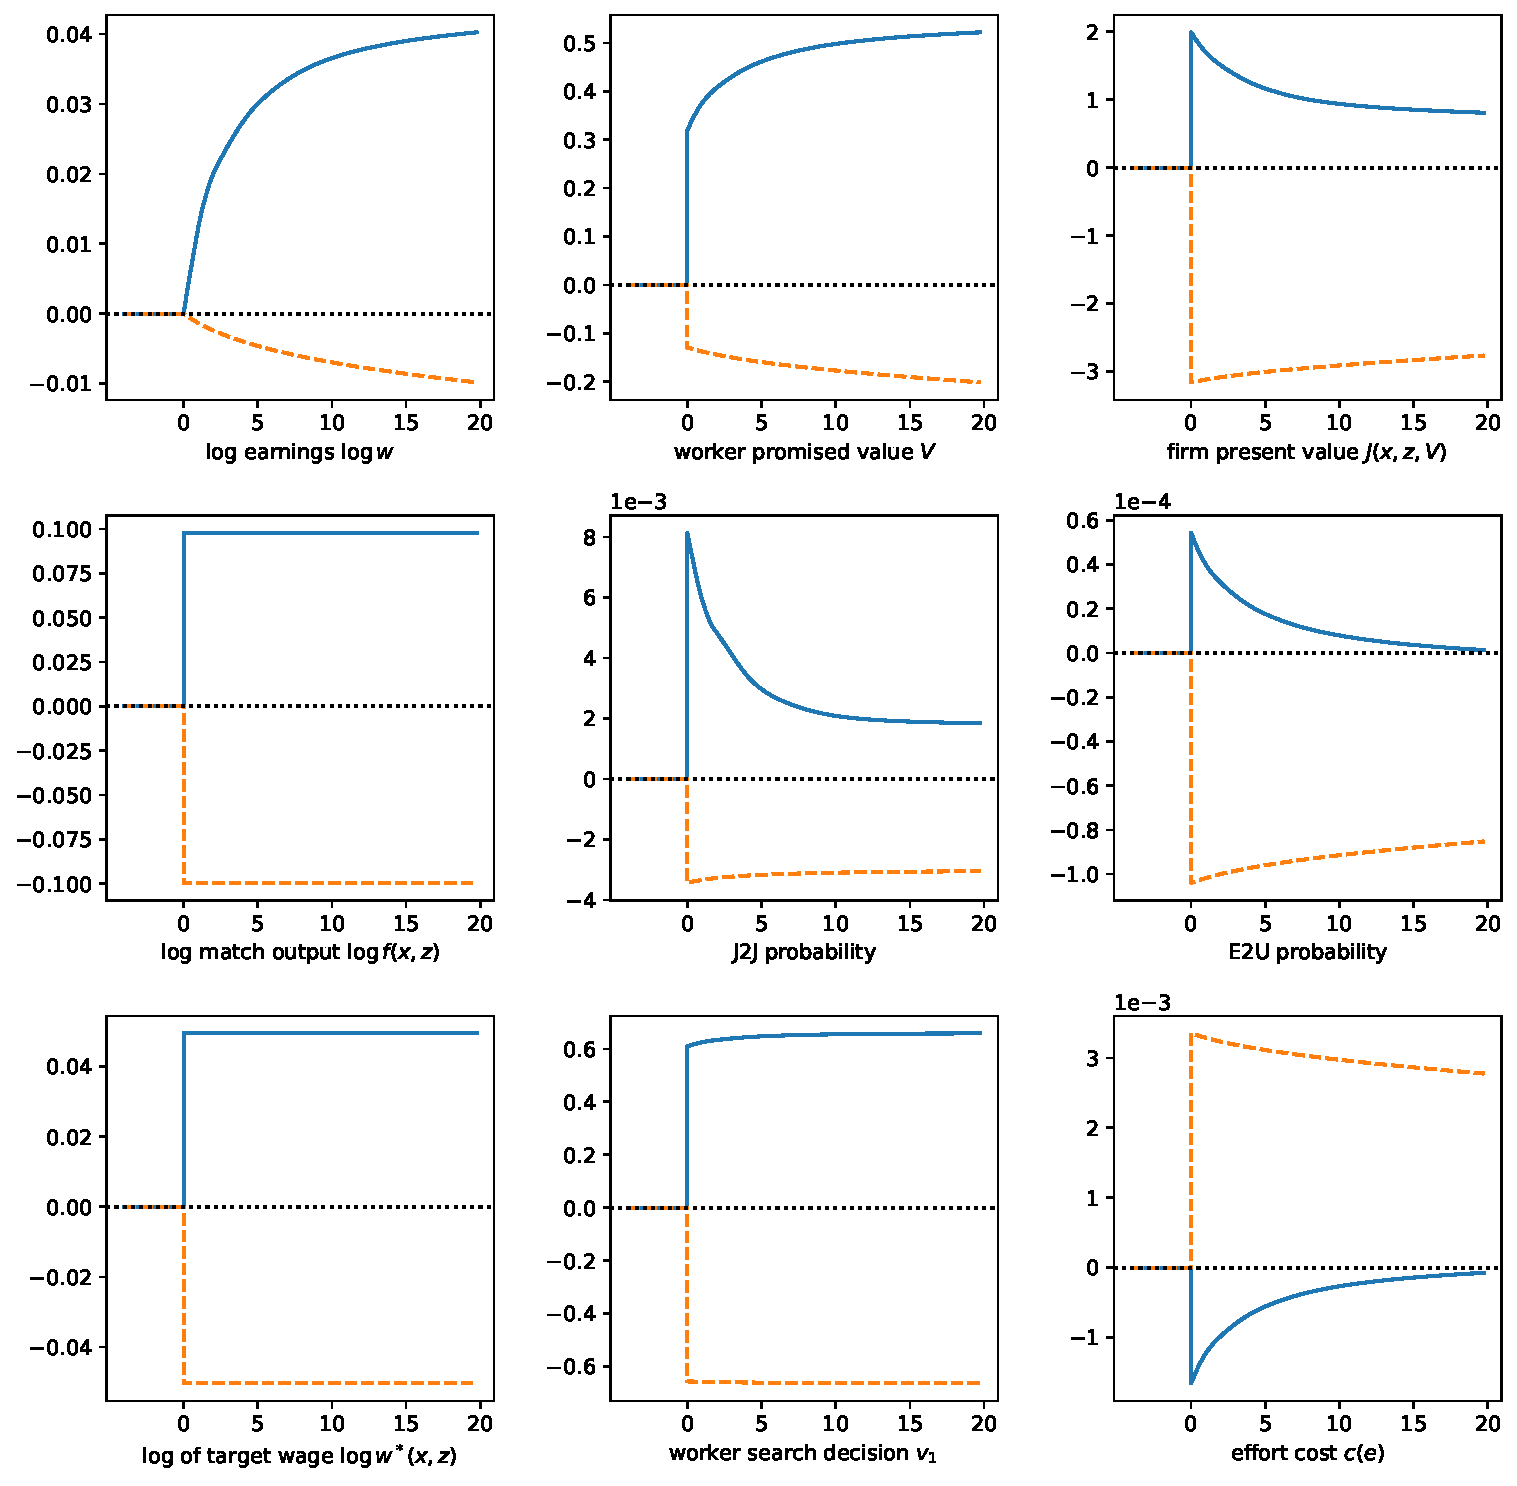
\includegraphics[width=0.8\textwidth]{figures/figure3-ir-xshock.pdf}
    \caption{Impulse response of a permanent shock to worker productivity $x$}
    \label{fig:impulse_response_x}
\end{figure}

\begin{figure}[htpb]
    \centering
    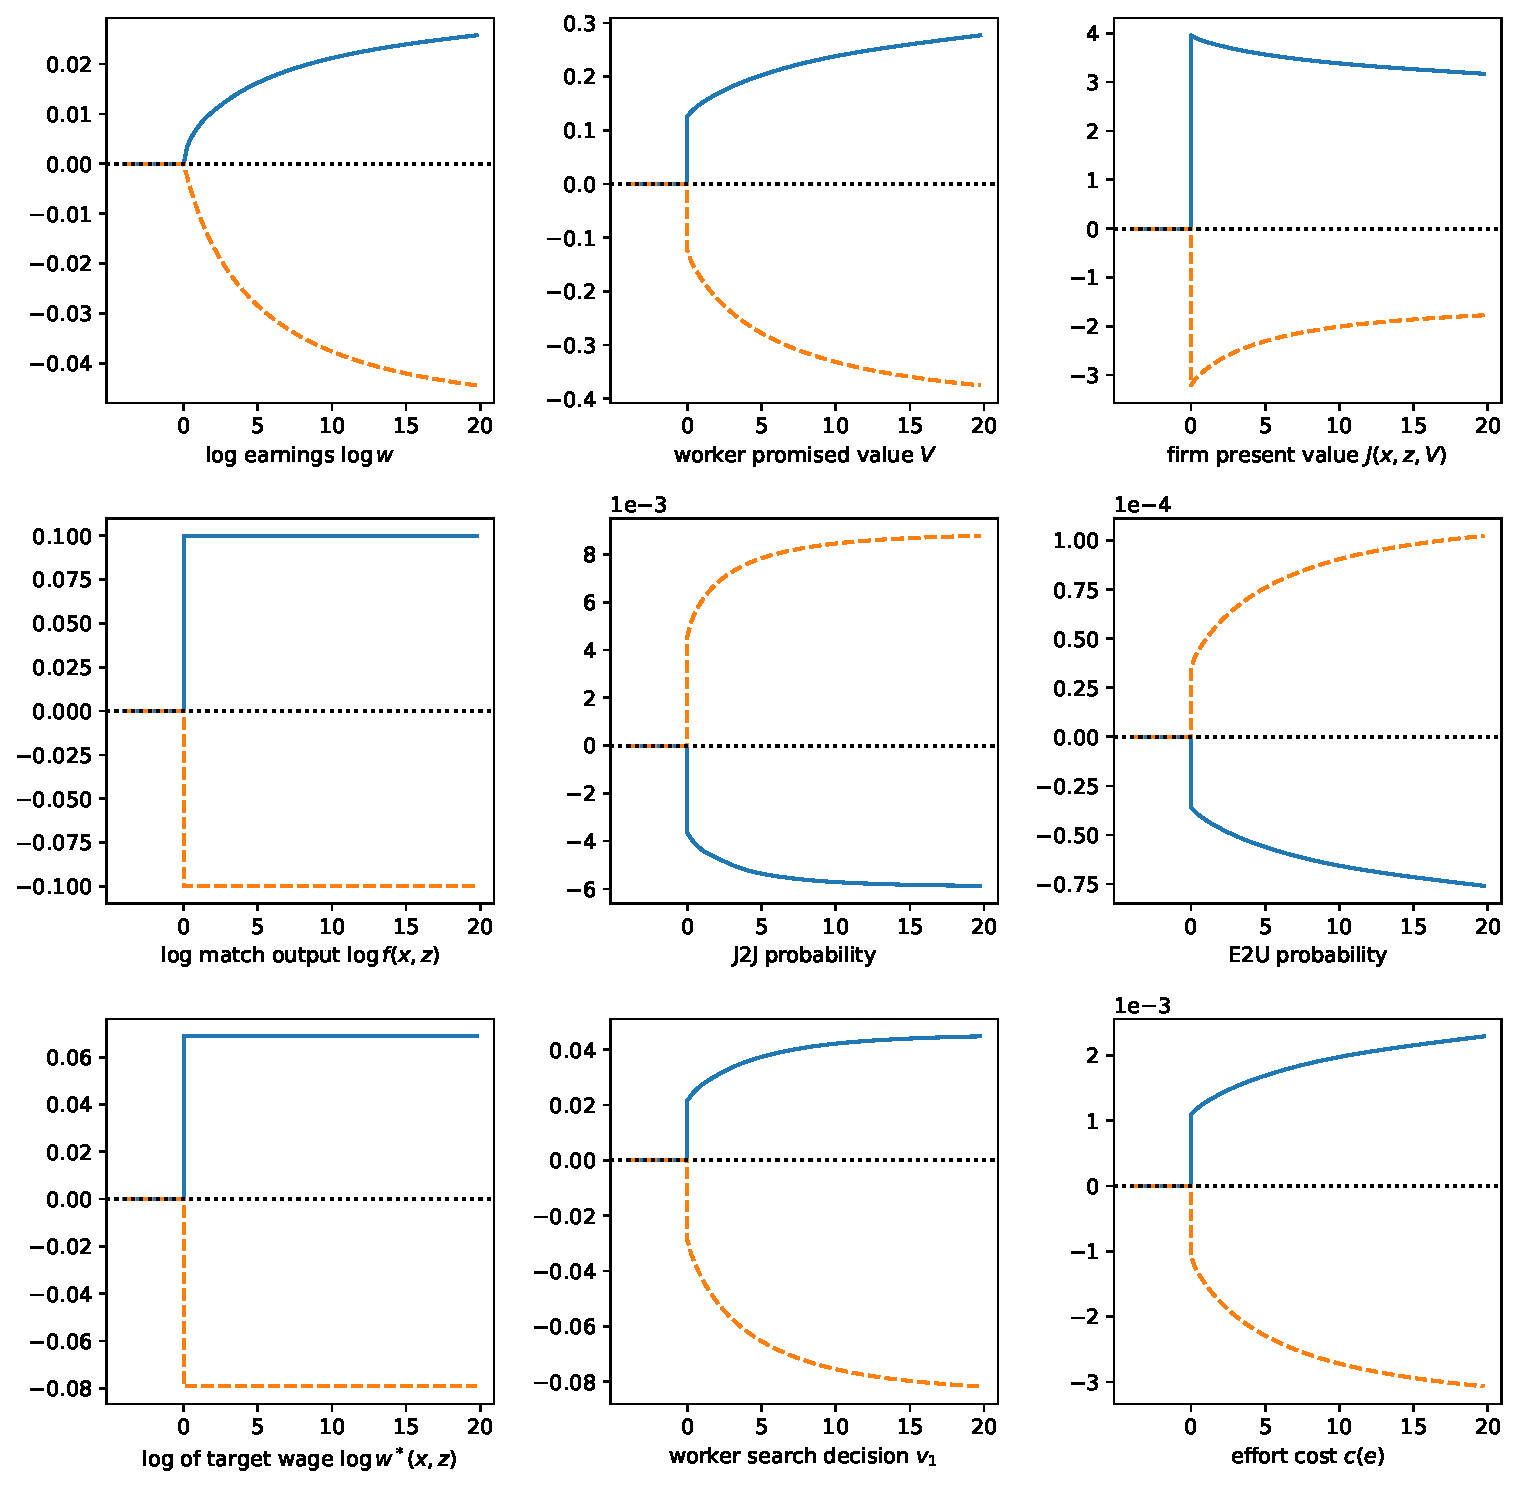
\includegraphics[width=0.8\textwidth]{figures/figure4-ir-zshock.pdf}
    \caption{Impulse response of a permanent shock to match quality $z$}
    \label{fig:impulse_response_z}
\end{figure}

\newpage

\section{Variance Decomposition}

\begin{table}[htpb]
    \caption{Level Variance Decomposition}
    \label{tab:level_variance_decomposition}
    \centering
    \begin{tabular}{l r r r r r r} 
        \toprule 
         & total & $x_0$ & $x_1$ & $z$ & other\\[4pt]
         & \multicolumn{5}{c}{overall}\\[-3pt]
         \cmidrule(lr){2-6}
        match output $f^a_{it}$ & $0.31$ & $11\%$ & $61\%$ & $24\%$ & $5\%$\\
        target wage $w^{*a}_{it}$ & $0.14$ & $32\%$ & $33\%$ & $31\%$ & $4\%$\\
        earnings $w^a_{it}$ & $0.14$ & $31\%$ & $7\%$ & $9\%$ & $53\%$\\[5pt]
         & \multicolumn{5}{c}{within individual, over time}\\[-3pt]
         \cmidrule(lr){2-6}
        match output $f^a_{it}$ & $0.08$ & $0\%$ & $18\%$ & $6\%$ & $2\%$\\
        target wage $w^{*a}_{it}$ & $0.03$ & $0\%$ & $10\%$ & $7\%$ & $1\%$\\
        earnings $w^a_{it}$ & $0.01$ & $0\%$ & $3\%$ & $3\%$ & $5\%$\\
        \bottomrule 
    \end{tabular}    
\end{table}

\begin{table}[htpb]
    \caption{Growth Variance Decomposition}
    \label{tab:growth_variance_decomposition}
    \centering
    \begin{tabular}{l r r r r r} 
        \toprule 
         & Total & U2E/E2U & J2J & $x_1$ & $z$\\
         \cmidrule(lr){2-6}
        $\text{Var}(\Delta\log f^a_{it})$ & 0.108 & -7.5\% & -4.3\% & 79.4\% & 18.2\%\\
        $\text{Var}(\Delta\log w^a_{it}) $ & 0.005 & 86.3\% & 13.4\% & 39.3\% & 13.7\%\\
        \bottomrule 
        \end{tabular}
\end{table}


\section{Pass-through}

\begin{table}[htpb]
    \caption{Pass-through Analysis}
    \label{tab:pass_through}
    \centering
    \begin{tabular}{l l r r} 
        \toprule 
         & mobility & $x_1$ shock & $z$ shock\\
         \cmidrule(lr){2-4}
        utility passthrough & outcome only & 0.26 & 0.10\\
         & yes & 0.24 & 0.16\\
        wage passthrough & yes & 0.32 & 0.39\\
         & no & 0.25 & 0.61\\
        \bottomrule 
        \end{tabular}        
\end{table}


\end{document}
